\chapter[Example Solutions]{EXAMPLE SOLUTIONS: \\ MESH INPUT TUTORIAL}
\label{examples}

Before proceeding with a description of the individual commands used by
{\sl FEAPpv} we describe 
some of the methods which may be used to
define an input data file. To do this we consider some sample finite element analysis
problems.
The first problem considered is a simple patch test in which all
the data is specified explicitly.  Later examples will illustrate how
{\sl FEAPpv} can generate missing data or use repeating similar parts to generate
a mesh.

\section{Example 1.  Patch Test Solution.}
\label{ex1}

The {\it patch test} is a
simple test which should be performed when first using any finite element
program 
(see Chapter 9 of \textit{The Finite Element Method: Its Basis \& Fundamentals}
by Zienkiewicz, Taylor and Zhu\scite{zt1n6}, for description
of patch test). The patch test
both ensures that the theory for the finite element formulation has been
correctly implemented and that installation of the analysis
system is also correct.  For a problem in linear elasticity one patch test
is uniform stress in the $x$ direction.  This condition may be
imposed on a square region divided into 4-elements and loaded by a constant
$x$-traction on the right side as shown in Figure \ref{fig1} (node 6 is
located at $y = 5$ units).  For a square
with side lengths 10 and a 10 unit
per length traction, the nodal forces on the boundary are 2.5 at the corners
and 5.0 at the midside.  The left side of the mesh is restrained so that
no $x$-direction displacements occur and the lower left corner is also
restrained in the $y$-direction.  These restraints prevent rigid body
motions as well as ensure that a correct solution to the constant stress
problem may be obtained.

\begin{figure}[ht!]
\centerline {\hfil 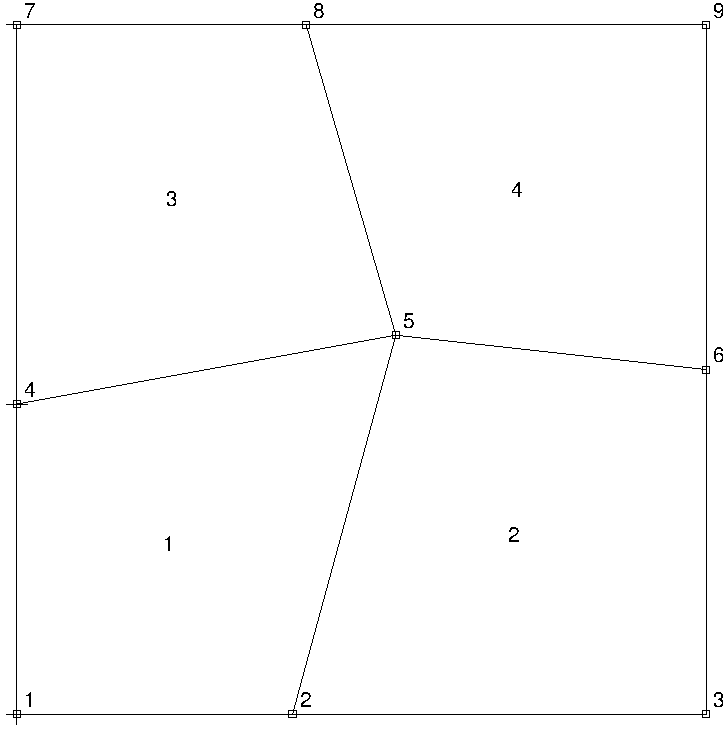
\includegraphics[width=2.3in]{figs/patch4} \hfil}
\caption{Patch Test Mesh}
\label{fig1}
\end{figure}
For  a linear elastic problem with the isotropic properties: Young's modulus
1000 and Poisson ratio 0.25, the plane strain solution has
displacements
$$ u = 0.009375 \, x  ~~;~~ v = - \, 0.003125 \, y$$
and stresses
$$ \sigma_{xx} = 1.0  ~~;~~ \sigma_{yy} = 0.0 ~~;~~ \sigma_{xy} = 0.0 ~~;~~
\sigma_{zz} = 0.25$$

The input data for {\sl FEAPpv} is prepared and placed in a file on disk.
It is recommended that the filename for the input data have a first
character of {\tt I}.  The filename should not exceed 128 characters.
The filename for the input data of the patch test will be
called {\tt Ipatch} for the discussion below.
When {\sl FEAPpv} is executed the names for other files will be assigned by 
replacing the first character by one indicating the type of file.  For
example, the file containing the description of the mesh and solution
results is called the {\it output} file and for the above choice
for input data will be named {\tt Opatch}.
The complete input data file for the patch test
problem is shown in Table \ref{tab1a} and a 
description for each part of this data follows.
Input records for {\sl FEAPpv} are free format.  Each data item
is separated by a comma and/or blank character(s).
If blank characters are used without commas, each data item {\it must} be
included.  That is multiple blank fields are not considered to be a zero.
Each data item is restricted to 15 characters (16 including the blank or
comma).

\begin{table}
\begin{verbatim}
       FEAPpv * * 4-Element Patch Test
         9,4,1,2,2,4
       MATErial,1
         SOLId
           PLANe STRAin
           ELAStic ISOTropic 1000.0 0.25
                         ! Blank termination record
       COORdinates
         1 0  0.0  0.0
         2 0  4.0  0.0
         3 0 10.0  0.0
         4 0  0.0  4.5
         5 0  5.5  5.5
         6 0 10.0  5.0
         7 0  0.0 10.0
         8 0  4.2 10.0
         9 0 10.0 10.0
                         ! Blank termination record
       ELEMents
         1 1 1 1 2 5 4
         2 1 1 2 3 6 5
         3 1 1 4 5 8 7
         4 1 1 5 6 9 8
                         ! Blank termination record
       BOUNdary restraints
         1 0 1 1
         4 0 1 0
         7 0 1 0
                         ! Blank termination record
       FORCes
         3 0 2.5 0.0
         6 0 5.0 0.0
         9 0 2.5 0.0
                         ! Blank termination record
       END
\end{verbatim}
\caption{Data for Patch Test}
\label{tab1a}
\end{table}

\begin{table}
\begin{verbatim}
       BATCh
         FORM residual
         TANGent
         SOLVe
         DISPlacement ALL
         STREss ALL
       END
       STOP
\end{verbatim}
\caption{Data for Patch Test}
\label{tab1b}
\end{table}

The input file {\tt Ipatch} consists of several data sets.  For
the patch test mesh given in Table \ref{tab1a} these are the commands
(shown without indentation in the table):
\begin{verbatim}
       FEAPpv * * 4-Element Patch Test
       MATErial
       COORdinates
       ELEMents
       BOUNdary restraints
       FORCes
       END
       BATCh
       END
       STOP
\end{verbatim}
{\sl FEAPpv} interprets only the first four characters of each command.  These
are shown as upper case letters to indicate the minimum amount which may be
used to identify each command.  Either upper case or lower case letters
may be used to identify each command.  Thus, 
{\tt MATE} or {\tt mate} may be used to identify the material property
data sets. After a {\tt FEAPpv} command and the control record,
the commands before the first {\tt END}
may be in any order and define the mesh for the problem. The commands
after the {\tt BATCH} describe the solution algorithm for the problem and
terminate with the second {\tt END} command.  Finally, the {\tt STOP}
command informs {\sl FEAPpv} that no more data exists.

The control record defines the size of finite element problem to be solved.
The first field defines the number of nodes ({\tt NUMNP}), the next field is the
number of elements ({\tt NUMEL}), followed by
the number of material sets ({\tt NUMMAT}),
the spatial dimension for the mesh ({\tt NDM}), the number of degrees of
freedom for each node ({\tt NDF}), and the maximum number of nodes on
any element ({\tt NEN}).  The patch test has a mesh with 9 nodes, 4 elements,
and 1 material set.  The problem is 2 dimensional, has 2 degrees of freedom
at each node, and each element has 4 nodes.

The first data set is identified by the {\tt MATE}rial command.  This record
also must contain a material set number (ranging from 1 to the maximum
number of sets needed).  The next records consist of commands which describe
the type of element (see Chapter \ref{elmlib}
for the types of elements included with
{\sl FEAPpv}) and the material parameters associated with the set.  The
data shown in Table \ref{tab1a}
indicates a {\tt SOLI}d (continuum) element is used,
the problem is plain strain and the material parameters are associated
with a linear elastic isotropic material.
Except for the element type record, other data may be in any order
and terminates with a blank record (comments are permitted on
records and begin with the exclamation point, "!", in column 3 or later).

The values of the nodal coordinates for the patch are specified using the 
{\tt COOR}dinate command.  Each record defines a node number, a generation
parameter, and the $x$ and $y$ coordinate
values.  Nodes may be in any order, but are shown in increasing order
in Table \ref{tab1a}.  Input terminates with a blank record.

The manner in which nodes are connected to form individual
finite elements and their association to the type of element and material
parameters is described by the data following the {\tt ELEM}ent command.
Each record defines the element number (which {\it must} be in increasing
numerical order), a generation parameter (to be described later), the
material data set associated with the element, and the list of nodes connected
to the element.  For the elements shown in Figure \ref{fig1} the node sequence
must start with a node at one vertex and then proceed with the nodes
on vertices traversed counter clockwise around the element.
Input terminates with a blank record.

The degree of freedoms for each node may have known applied loads (nodal
forces) or may be restrained to satisfy specified nodal displacements.
In {\sl FEAPpv} all degree of freedoms are assumed to have specified loading
applied unless a restraint code is set.  The {\tt BOUN}dary restraint
command may be used to assign restraints to degree of freedoms which are
to have specified displacements.
Each record defines a node number, a generation parameter,
and the restraint codes for each degree of freedom associated with
the node. A non-zero value for the restraint code 
indicates that the associated degree of freedom must satisfy a specified
nodal displacement value (default is zero); whereas, a zero restraint
code indicates the associated degree of freedom has a specified nodal
force (also zero by default).  Thus, for the data shown in Table \ref{tab1a},
node 1 has both the $u$ and $v$ displacements restrained; nodes 4 and 7
have the $u$ displacement restrained and the $y$ force specified.  All
other nodes have both the $x$ and the $y$ forces specified since no
restraints are specified.
Input terminates with a blank record.

It is evident from the remaining data that
no data is provided to impose non-zero displacements (methods to input
non-zero values are described in Section \ref{bc}); however, data is given to
impose non-zero forces using the {\tt FORC}e command.  
Each force record defines a node number, a generation parameter,
and the force values for each degree of freedom associated with
the node.  Thus, for the data given in Table \ref{tab1a}, nodes 3 and 9 have
$x$ force values of 2.5 units and node 6 has an $x$ force value of 5.0
units. Input terminates with a blank record.

The final command after the force values is the {\tt END} command which
terminates input of the data describing the finite element mesh.

The set of commands shown in Table \ref{tab1b}
define the solution algorithm to be used in solving the
problem.  The execution is initiated by the {\tt BATC}h command
(alternatively, it
is possible to perform an interactive execution where users enter each
command as needed, see next example and
Chapter \ref{command}).  The {\tt FORM} command instructs {\sl FEAPpv}
to form the residual for the equilibrium equations written as:
$$\B{R} ( \B{u} ) ~=~ \B{F} ~-~ \B{P}( \B{u} )$$
where $\B{F}$ is the vector of applied nodal forces,
$\B{u}$ is the vector of nodal displacements, and
for a static linear elastic problem $\B{P}$ is defined as
\begin{equation}
\B{P} ~=~ \B{K} \, \B{u}
\end{equation}
in which $\B{K}$ is the stiffness matrix.
A solution to the problem is defined by requiring the residual to be zero.
In {\sl FEAPpv} the solution may be computed using Newton's method which solves
a sequence of linear problems.
Thus, the {\tt TANG}ent command
requests the tangent matrix to the residual about the current solution state,
$\B{u}$ (at start of execution
the value is zero)
where the tangent matrix is defined as:
\begin{equation}
\B{K}_{tang} ~=~ - \, \frac{\partial \B{R}}{\partial \B{u}}
\end{equation}
Thus, for a linear elastic
static problem the tangent matrix is just $\B{K}$.
The {\tt SOLV}e command instructs {\sl FEAPpv} to solve
the incremental (Newton) equations
\begin{equation}
\B{K}_{tang} \, \Delta \B{u} ~=~ \B{R}
\end{equation}
and to update the solution as
\begin{equation}
\B{u} ~ \leftarrow ~ \B{u} ~+~ \Delta \B{u}
\end{equation}
For a linear problem this solution sequence should converge in one iteration;
thus, the residual would be zero if the command {\tt FORM} is given again.

At this point {\sl FEAPpv} has computed the solution; however, it is necessary
to issue additional commands to output the values for each type of solution
quantity.
The {\tt DISP}\-lace\-ment command instructs {\sl FEAPpv} to output values for
the nodal generalized displacement parameters associated with each nodal
degree of freedom (for linear elasticity using solid elements these are
the values of the $u$ and $v$ displacements at a node).
The option {\tt ALL} requests the displacement
values for all active nodes (see manual
pages in Appendix A for other options).  Similarly, the command
{\tt STRE}ss, {\tt ALL} requests output values for
stresses within all the active elements (see Appendix A for other options).
All output is placed in the output file.

\section{Example 2.  Truss Problem Solution.}
\label{ex2}

As a next example for the use of {\sl FEAPpv}, consider a simple truss problem.
The mesh, nodal and element numbers, loading, restraints, and material
properties are shown in Figure \ref{fig2}.

\begin{figure}[ht!]
\centerline {\hfil 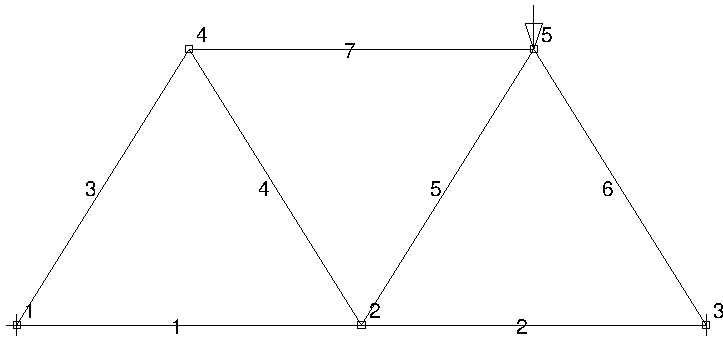
\includegraphics[height=2.3in]{figs/truss4} \hfil}
\caption{Mesh for Truss Example}
\label{fig2}
\end{figure}
The complete data file for the problem is shown in Table \ref{tab2} and a 
description for each part of this data follows.

\begin{table}
\begin{verbatim}
       FEAPpv * * 2-D Truss Problem
         5 7 2 2 2 2
       MATErial,1
         TRUSS
           ELAStic ISOTropic 1000.0
           CROSs SECTion     10.0
                         ! Blank termination record
       MATErial,2
         TRUSS
           ELAStic ISOTropic 1000.0
           CROSs SECTion     5.0
                         ! Blank termination record
       COORdinates
         1 0 0.0 0.0
         2 0 200.0 0.0
         3 0 400.0 0.0
         4 0 100.0 160.0
         5 0 300.0 160.0
                         ! Blank termination record
       ELEMents
         1 0 1 1 2
         2 0 1 2 3
         3 0 1 1 4
         4 0 2 2 4
         5 0 2 2 5
         6 0 1 3 5
         7 0 1 4 5
                         ! Blank termination record
       BOUNdary restraints
         1 0 1 1
         3 0 0 1
                         ! Blank termination record
       FORCe
         5 0 0.0 -10.0
                         ! Blank termination record
       END
\end{verbatim}
\caption{Data for Truss Analysis Problem}
\label{tab2}
\end{table}

The control record indicates the mesh has 5 nodes, 7 elements, 2 
material sets. It is a 2 dimensional problem with 2 degrees of freedom at each
node and 2 nodes for each truss element.

The {\tt MATE}eral property sets for all members
are identical except for the cross sectional
area of the members (the first numerical field on the {\tt CROS}s
{\tt SECT}ion record). Two types are indicated: Set 1 has an area of 10 units
while set 2 has an area of 5 units.

The coordinates are input as for the patch example described above.  Element
properties are also input in a similar way; however, note that the material
property set in the third field now is set to either 1 or 2 depending on
whether the cross section has 5 or 10 units of area.
Boundary restraint conditions are imposed so that node 1 is restrained
to have zero $u$ and $v$ displacements while node 3 has only a restrained
$v$ displacement.  Finally, a single load in the vertical direction
with magnitude -10.0 is applied to node 5.

This problem requests an {\tt INTE}ractive mode of solution.  In the interactive
mode users must give the solution commands needed for each solution step.
For example, when the command {\tt FORM} is given {\sl FEAPpv} will compute
the residual and then prompt for another command input.  Similarly, 
giving the commands for output will display the request on the screen and
also place the information in the output file.

\section{Example 3. Circular Disk Subjected to Point Loading}
\label{ex3}

The next problem considered is a circular disk loaded by
two concentrated forces of 10 units each
directed along a diagonal (see Figure \ref{fig3}). The material
of the disk is assumed to be linearly elastic.  Furthermore, for simplicity
we consider the loads to be slowly applied so that inertial effects may
be ignored.  Thus, the model to be solved is a simple linear elasto-static
problem.  Since the loading is symmetric and we assume the material to be
isotropic (and thus also symmetric), it is only necessary to construct a mesh
for one quadrant of the circular disk.

This problem has curved boundaries and requires a general mesh
to define the finite element solution, thus, more details
are described for the input data options available in {\sl FEAPpv}.

\begin{figure}[ht!]
\centerline {\hfil 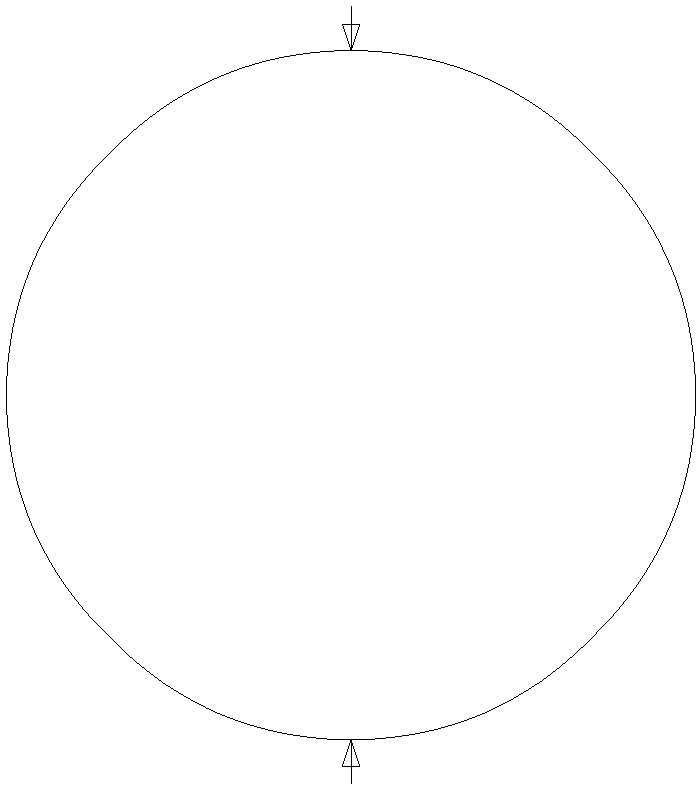
\includegraphics[width=1.6in]{figs/fig1} \hfil}
\caption{Circular Disk with Point Loading}
\label{fig3}
\end{figure}

In the two dimensional capabilities included in
{\sl FEAPpv}, the solid elements permit an analyst to use elements with
between 3 and 9 attached nodes.  A 3-node element is a plane triangle
with nodes located at each vertex.  A 4-node element is a quadrilateral with
nodes at each vertex.  A 9-node element is quadrilateral in shape but
may have curved sides defined by nodes located in the mid part of
each edge, as well as one
additional node in the interior.  Omitting some midside nodes and/or
the center node produces quadrilateral elements with between 5 and 8 nodes.

Let us assume that a mesh will be constructed using 4-node
quadrilateral elements.  The nodes are defined by a sequence
starting with {\it Node 1} and concluding with the maximum number {\it
Node NUMNP}.
The elements also are defined by a sequence starting with {\it Element 1}
and concluding with {\it Element NUMEL}.
A 4-node quadrilateral element is defined by
the node numbers associated with each vertex.  A simple
mesh for one quadrant of the disk is shown in Figure \ref{fig2}.
The figure shows
the numbers associated with each node and element.
This mesh has 19 nodes ({\tt NUMNP} = 19) and 12 elements ({\tt NUMEL} = 12).

\begin{figure}[ht!]
\centerline {\hfil 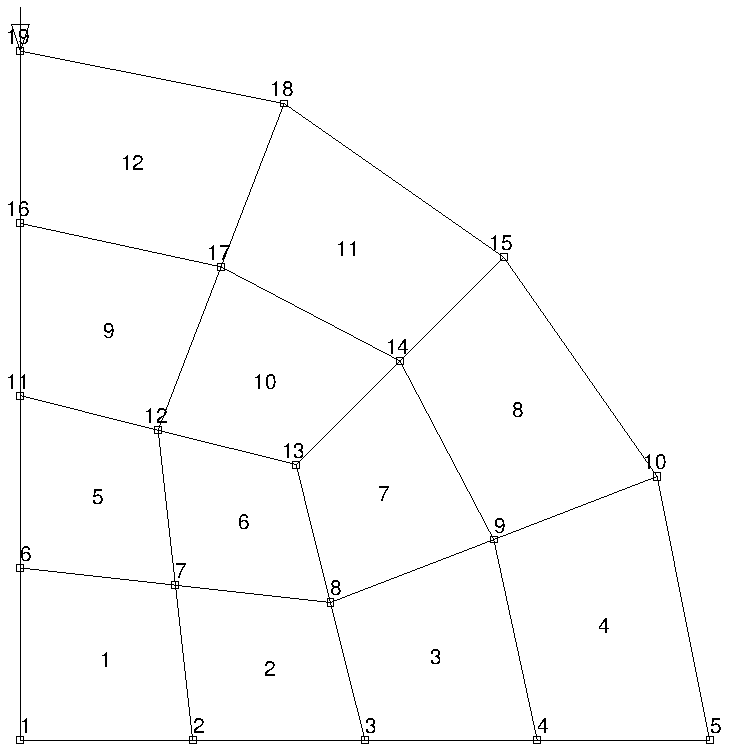
\includegraphics[width=2.8in]{figs/fig2} \hfil}
\caption{Finite Element Mesh for Circular Disk with Point Loading}
\label{fig4}
\end{figure}

The control data for the mesh shown in Figure \ref{fig4} is:
\begin{verbatim}
             FEAPpv * * Example 1.  Circular Disk: Basic inputs
             19 12 1 2 2 4
\end{verbatim}
The remainder of the finite
element mesh is described using the data set concepts introduced in the
previous examples.

There are options to specify the number and coordinates for each
nodal point.  The one used to this point is the {\tt COORdinate} option.
Since only the first 4 characters of each command
are interpreted by {\sl FEAPpv}, the use of {\tt COOR} or {\tt COORDINATE}
produces identical results.
After the {\tt COOR} command individual records defining each nodal point
and its coordinates (in the present case the $x_1$ and $x_2$ coordinates)
are specified as:

\begin{verbatim}
             N, NG, X-1, X-2
\end{verbatim}
where
$$\vbox { \halign { # \hfil && \quad # \hfil \cr
\begin{center}
\begin{tabular{ l l }
N   & Number of nodal point. \\
NG  & Generation increment to next node. \\
X-1 & value of x-1 coordinate. \\
X-2 & value of x-2 coordinate.
\end{tabular}
\end{center}
Thus, for the mesh shown in Figure \ref{fig2},
the coordinate data may be specified as:
\begin{verbatim}
             COORdinates
              1   1   0.0000       0.0000
              5   0   1.0000       0.0000
              6   1   0.0000       0.2500
              8   1   0.4500       0.2000
             10   0   0.9239       0.3827
             11   1   0.0000       0.5000
             13   1   0.4000       0.4000
             15   0   0.7010       0.7010
             16   0   0.0000       0.7500
             17   0   0.2913       0.6869
             18   0   0.3827       0.9239
             19   0   0.0000       1.0000
                         ! Blank termination record
\end{verbatim}
The missing node numbers and their coordinate values are generated
using linear interpolation on the NG generation sequence given.
Thus, the first pair of records also generates nodes 2 to 4 with coordinates:
\begin{verbatim}
              2   0.2500       0.0000
              3   0.5000       0.0000
              4   0.7500       0.0000
\end{verbatim}
Comments may be appended after the second character of
any line by using an exclamation followed by the text.
Other options to define coordinates are discussed later.

There are also different options which may be used to generate the
element connection data.  One is the {\tt ELEM}ent command which
is given as:
\begin{verbatim}
             N, NG, MA, N-1, N-2, N-3, N-4
\end{verbatim}
where
\begin{center}
\begin{tabular{ l l }
N   & Number of element. \\
NG  & Generation increment for node numbers. \\
MA  & Material identifier associated with element. \\
N-1 & Node number for first vertex. \\
N-2 & Node number for second vertex. \\
N-3 & Node number for third vertex. \\
N-4 & Node number for fourth vertex.
\end{tabular}
\end{center}
Any vertex of the quadrilateral may be used to define {\tt N-1}.
The remainder, however, should be specified using a counter clockwise
sequencing around the nodes as shown in Figure \ref{fig4a}.

\begin{figure}[ht!]
\centerline {\hfil 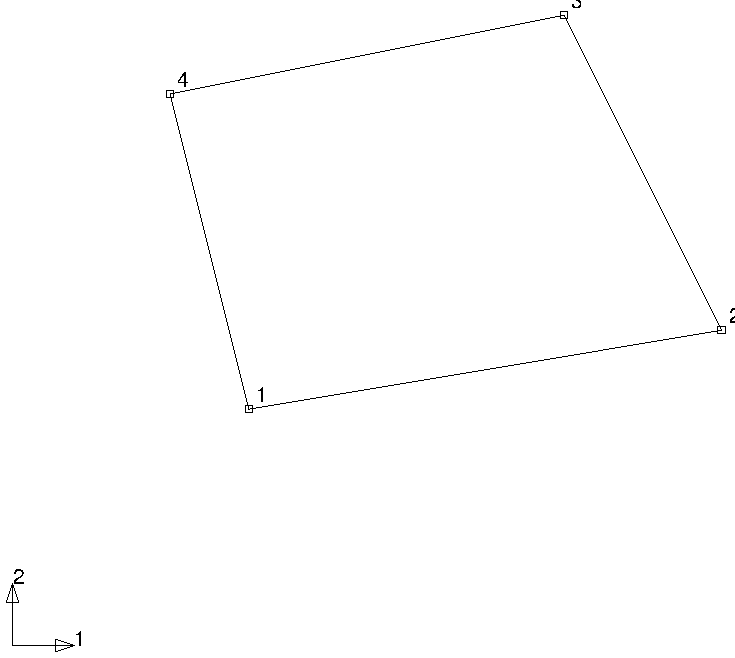
\includegraphics[width=2.8in]{figs/fig1a} \hfil}
\caption{Node Sequencing for 4-node Quadrilateral}
\label{fig4a}
\end{figure}

The element connection data for the example problem is given by:
\begin{verbatim}
               ELEMents
                1 1 1  1  2  7  6
                5 1 1  6  7 12 11
                9 1 1 11 12 17 16
               10 1 1 12 13 14 17
               11 1 1 14 15 18 17
               12 0 1 16 17 18 19
                         ! Blank termination record
\end{verbatim}
Elements within a data set must be in order; however, gaps may occur
and missing elements will be generated.
The second field in each of the element records defines the
increment to apply to nodes in order to generate missing elements.  Thus,
from the first two pairs of records it is evident that elements 2, 3, and 4
are missing.  The generation increment to apply to the nodes on element 2 is
specified as 1 on the element 1 record\footnote{If the field is
omitted a default value of 1 is assumed.}.
Accordingly, the generated elements
will have the following sequence of nodes.
\begin{verbatim}
                2      2  3  8  7
                3      3  4  9  8
                4      4  5 10  9
\end{verbatim}
The material identifier
number will be the values specified in the third field and
for the data above will be 1 for all generated elements (the material
identifier for generated elements
is taken from the first record of each generation pair).

Multiple {\tt ELEM}ent sets may be used or {\tt ELEM}ent may be combined
with other options (e.g., {\tt BLOC}k type generations).

To complete the problem specification it is necessary to impose constraints
on the nodal displacements along the symmetry axes, specify the applied
concentrated load, and define the material set properties.  A set of commands
which accomplish this is given by
\begin{verbatim}
             BOUNdary restraint codes
              1 1  1 -1
              5 0  0  1
              6 5 -1  0
             19 0  1  0
                         ! Blank termination record
\end{verbatim}
\begin{verbatim}
             FORCes on nodes
             19 0 0 -5.0
                         ! Blank termination record
\end{verbatim}
\begin{verbatim}
             MATErial,1
             SOLId
             ELAStic ISOTropic 10000 0.25  ! E and nu
             DENSity data      0.1         ! rho
             QUADrature data 2 2
                         ! Blank termination record
             END
\end{verbatim}
The set of records following the {\tt BOUN}dary code command
imposes the necessary restraints on nodes. A non zero
restraint code implies the value of the corresponding displacement component
will have specified values (default values are 0.0);
whereas, a zero code (the default
restraint code value) indicates the component is unknown and must be computed.
The inputs use generation, similar to the {\tt COOR} data.  Thus the first
pair of records will also generate restraints for nodes 2, 3, and 4.  A negative
or zero code will propagate to the generated node, whereas a positive code
will become a zero values on the generated nodes.  Thus the first pair
will generate a set of restraints such that the first displacement
component ($u_1$) will be an unknown and the second component ($u_2$) will
be set to a specified value.
The last pair of records also generates restraints for the first degree
of freedom of nodes 11 and 16.

For degree of freedoms with zero restraint codes {\sl FEAPpv} will add a force
value to each node (default is 0.0);
whereas, for non zero restraint codes {\sl FEAPpv} will
impose a displacement value (default is 0.0).  Non zero forces may
be specified using a {\tt FORCe} command (other options also exist
as described later).  Non zero displacements may be specified using
a {\tt DISPlacement} command (again, other options exist).
Thus, for the example problem
a concentrated load ($F_2 = -5$) is applied on node 19 by the {\tt FORCe}
command set shown above.
The {\tt MATErial} record specifies the set number as 1.  The
next record requests the {\it SOLId} element type (See Chapters \ref{elmlib}
and \ref{matmods} for
additional information on types of elements and material models permitted).
The third record defines the material constitution as isotropic linear
elastic and sets the parameters
as $E = 1000$, $\nu = 0.25$.
The fourth record sets the material density as $\rho = 0.1$.
The fifth record specifies a $2 \times 2$ Gauss quadrature
to compute arrays and output element results.
The input of material parameters terminates with a blank record.  The data
following the {\tt SOLId} specification may be in any order.  Also any data
not needed may be omitted.  Since the disk analysis is quasi-static the
material density is unnecessary and could be omitted.  Also default quadrature
values will be used if this record is omitted.  For the current analysis the
minimum material data is:
\begin{verbatim}
       MATErial,1
         SOLId
         ELAStic ISOTropic 10000 0.25  ! E and nu
                         ! Blank termination record
\end{verbatim}

The {\tt END}
command signals {\sl FEAPpv} that the specification of the mesh and initial
loading conditions is complete.  An mesh may be modified during
the solution phase by re-entering {\tt MESH} generation or by manipulating
the mesh to merge parts using the {\tt TIE} command
or setting boundary conditions to satisfy {\tt LINK} or {\tt ELINk} conditions.
\vskip 0.2in

We next describe some of the other options which are available
to generate and/or manipulate a mesh.
Again we consider the example problem to make the discussion specific.

The preceding format to generate the data for a finite element
mesh for the example problem is quite
restrictive.  If it is desired to increase the number of nodes and
elements it is necessary to restart the process from the very beginning.
Thus, we now consider options for describing the mesh which permit the
problem to be described more easily, as well as, permit the number of
nodes and elements to be increased or decreased.

{\sl FEAPpv} has some powerful options which permit the generation of
problems in a form amenable to refinement.  For example, the control
record pair may be specified with 0 nodes, 0 elements, and/or 0 materials
indicated.  {\sl FEAPpv} will
use the subsequent data to compute the number of nodes, elements, and material
sets in the
mesh\footnote{If user mesh functions are employed this feature may
not work correctly}.  Accordingly, it is possible to use:
\begin{verbatim}
       FEAPpv * * Example 1.  Circular Disk: Block inputs
       0 0 0 2 2 4
\end{verbatim}
Without additional features this is of little merit.  However, nodes
and elements may be generated using a {\tt BLOCk} command as:
\begin{verbatim}
       PARAmeter
         m = 2
         n = 2
                          ! End of parameters
        BLOCk 1
         CARTesian,m,n,1,1,1
           1  0.0  0.0
           2  0.5  0.0
           3  0.4  0.4
           4  0.0  0.5
                          ! Blank termination record
\end{verbatim}
A {\tt BLOCk}  command uses a regular subdivision of the parent master
element shown in Figure \ref{fig4} to describe the mesh within its perimeter.
In Figure \ref{fig4} the coordinate directions 1 and 2 are local axes for
the {\tt BLOCk} generation (i.e., the natural coordinates for an isoparametric
master element). Using this convention, {\tt BLOCk 1} is described
by a 4 node quadrilateral master element whose coordinates are specified
as shown above.  The first record states that the master element coordinates
will be specified in Cartesian form (other options are {\tt POLAr} and
{\tt SPHErical}), the block will be divided into
$m$ subdivisions in the 1 direction and $n$ subdivisions in the $2$
direction (an $m \times n$ mesh of
quadrilaterals), with the first node, element, and material set
numbers set to 1. The values for $m$ and $n$ are assigned {\it prior} to the
{\tt BLOCk} specification using the {\tt PARAmeter} command followed by
the description of parameters.  Each parameter may only be one
character between {\tt a} and {\tt z} ({\sl FEAPpv} converts all data to lower
case internally, hence only 26 parameters are available for use at any one
time.  Parameters may, however, be redefined at later stages of the data.

\begin{figure}[ht!]
\centerline {\hfil 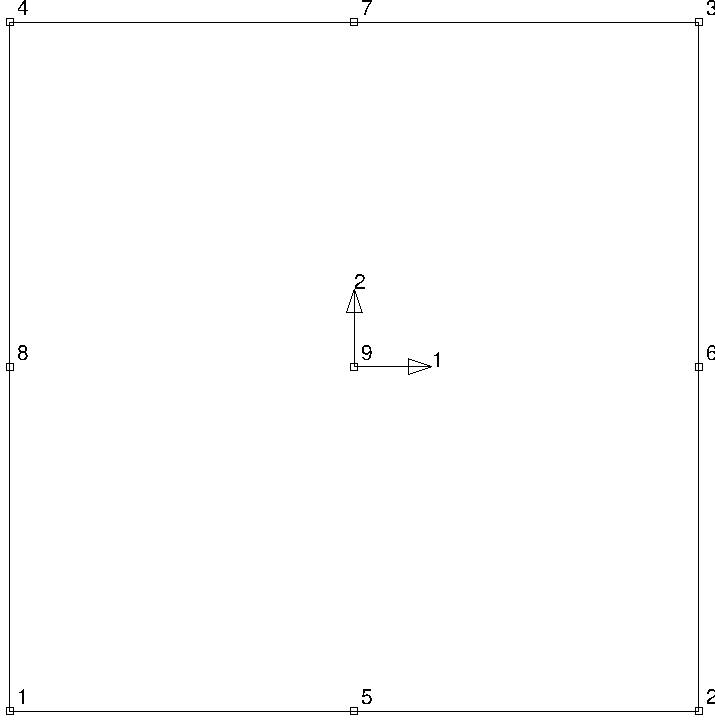
\includegraphics[width=2.8in]{figs/fig3a} \hfil}
\caption{Node Sequence to Define Master Nodes on a Block}
\label{fig5}
\end{figure}

Parameters for the sine and cosine of the angles at
the middle of the circular part of blocks are defined by:
\begin{verbatim}
       PARAmeters
         p = atan(1.)
         s = sin(0.5*p)
         c = cos(0.5*p)
                          ! Blank termination record
\end{verbatim}
The additional blocks needed to define the circular disk then may be given as:
\begin{verbatim}
       BLOCk 2
         CARTesian,n,n
           1 0.5   0.0
           2 1.0   0.0
           3 0.701 0.701
           4 0.4   0.4
           6 c     s
                          ! Blank termination record
\end{verbatim}
\begin{verbatim}
       BLOCk 3
         CARTesian,n,n
           1 0.4   0.4
           2 0.701 0.701
           3 0.0   1.0
           4 0.0   0.5
           6 s     c
                          ! Blank termination record
\end{verbatim}
The {\tt PARAmeter} command also permits arithmetic calculations
to be performed (see Chapter \ref{record} for further information).
In the above, the parameter {\tt p} is set to
$0.25 \pi$ (i.e., 45 degrees) and {\tt s} and {\tt c}
are the sin and cosine of 22.5 degrees.
The second and third blocks are also $2 \times 2$ meshes of quadrilaterals since
the value of {\tt n} has not been changed; however, each of these blocks are
described on an element with one edge curved along the circular boundary
of the disk.  Note also, that after defining the initial generation
sequence for the node and element numbers on the first block all others
have zero numbers. {\sl FEAPpv} will be able to compute the number for
the first node and element of each block so that the final mesh has 12
elements and 27 nodes (it is necessary to merge the blocks to produce
a mesh with only 19 active nodes needed to define the problem).

\begin{figure}[ht!]
\centerline {\hfil 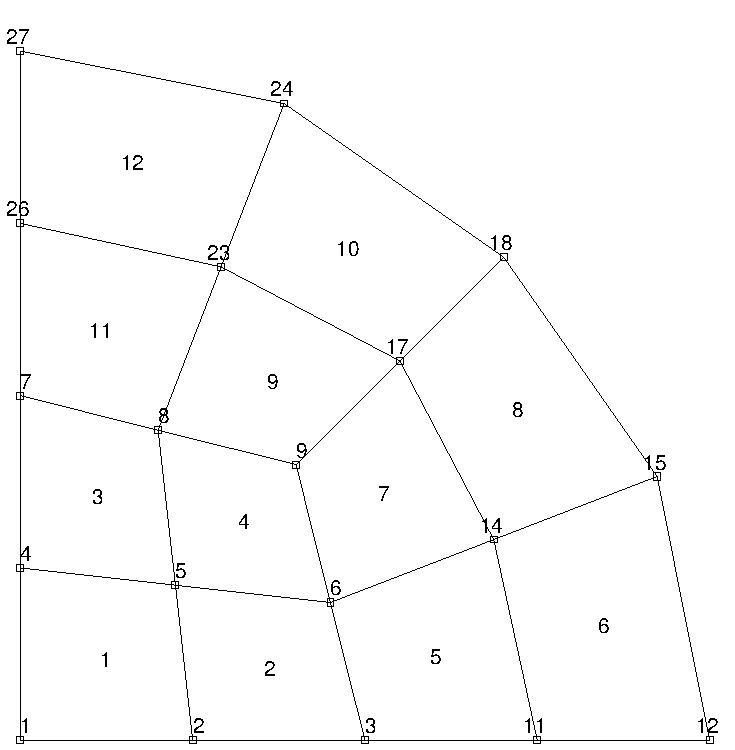
\includegraphics[width=2.8in]{figs/fig3} \hfil}
\caption{Finite Element Mesh for Circular Disk using Block Commands and Merging}
\label{fig6}
\end{figure}

The boundary conditions and applied nodal load may also be defined such that
it is not necessary to know node numbers by using {\tt EBOUndary} (for
edge boundary specification) and {\tt CFORced} commands
(for coordinate point force loading), respectively.  Accordingly,
\begin{verbatim}
       EBOUndary        ! Edge boundary restraints
         1 0.0 1 0
         2 0.0 0 1
                        ! Blank termination record
       CFORce           ! Coordinate specified forces
         NODE 0.0 1.0  0.0 -5.0
                        ! Blank termination record
       MATErial,1
         SOLId
         ELAStic ISOTropic 10000 0.25
         DENSity data      0.10
         QUADrature data 2  2
                        ! Blank termination record
       END
       TIE              ! Tie nodes with same coordinates.
\end{verbatim}
accomplish these steps and complete the description for the mesh
and its material properties.
Note particularly, the {\tt TIE} command following the generation of
the mesh.  This command will merge the three blocks to form a
mesh which is equivalent to the original mesh (however, this mesh has
different numbering for nodes and elements than the first mesh generated).
The numbers for the active nodes after the merge and the element numbers
produced by the block commands are shown in Figure \ref{fig6}.
The advantage of this form, however, is the ease by which the mesh
can be refined.  Indeed by assigning the parameter {\tt n} (and $m$) a value
of 5, one obtains a mesh with 75 elements as shown in Figure \ref{fig7}.

\begin{figure}[ht!]
\centerline {\hfil 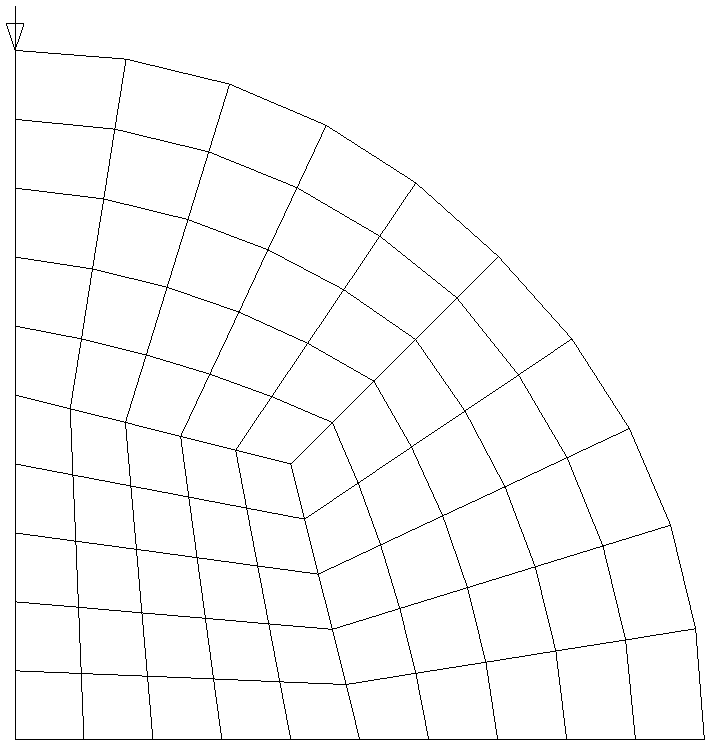
\includegraphics[width=2.8in]{figs/fig4} \hfil}
\caption{Mesh for Circular Disk. 75 Elements}
\label{fig7}
\end{figure}

Since the boundary conditions are associated with an edge, all nodes
which lie on the edge will be identified and restrained.  Similarly,
the node with the specified coordinates will be identified for the
applied $F_2 = -5.0$ force.
Additional details on options for the {\tt CFORce} command are given in the
mesh user manual pages in Appendix A.

Once the mesh is described the problem may be solved using
the solution command language.  Two modes of execution are available:
A batch mode where {\sl FEAPpv} enters a solution mode and processes all data
without user intervention; and an interactive mode where the user
issues each command or command group and receives prompts for additional data.
An analysis may use multiple batch and/or interactive solutions in the same
analysis.  To enter a batch execution the user inserts a command {\tt BATCh}
after the mesh {\tt END} record (and any other commands which manipulate
the mesh, e.g., {\tt TIE}), whereas to enter an interactive mode the
command {\tt INTEractive} is inserted.  The {\tt BATCh} execution command
must be immediately followed by the other solution commands and terminates
with an {\tt END} command.  To perform a batch mode
static (steady state) solution for the example problem the commands
\begin{verbatim}
       BATCh
         TANGent         ! Form tangent  (K)
         FORM            ! Form residual (R)
         SOLVe           ! Solve K*du = R
       END               ! End of batch execution
\end{verbatim}
may be included in the input data file after the {\tt TIE} command.
Alternatively, the command
\begin{verbatim}
       INTEractive
\end{verbatim}
may be included and the other commands given sequentially after receiving
the
\begin{verbatim}
       Macro 1.>
\end{verbatim}
prompt.  With either mode {\sl FEAPpv} process the sequence of commands to produce
a solution; however, no report of the results is provided unless specifically
requested.  To output all the nodal displacement values for the current
solution state the command
\begin{verbatim}
       DISPlacement,ALL
\end{verbatim}
may be given.  Similarly, the commands
\begin{verbatim}
       STREss,ALL
       REACtion,ALL
\end{verbatim}
produce outputs for all the element variables (stresses and any other values
included in the element output section) and reactions for all the nodes.
The order of output is controlled by the order of issuing the commands.  If the
solution is converged then nodal reactions should be zero (numerically) for
all degree-of-freedoms which are not restrained.  Restrained degree-of-freedoms
report the reaction force necessary to impose the specified
displacement constraint.

Alternatively, graphical outputs may be requested.  For example, the
commands
\begin{verbatim}
       PLOT,MESH
       PLOT,LOAD,,-1
\end{verbatim}
produce the results shown in Figure \ref{fig7}.
Contour plots are also possible.
Shaded contours for the vertical displacements are shown in Figure \ref{fig8}
and are obtained using the command
\begin{verbatim}
       PLOT,CONT,2
\end{verbatim}
Additional information on solution and plot commands is included in
Chapters \ref{command} and \ref{plot}, respectively.

\begin{figure}
\centerline {\hfil 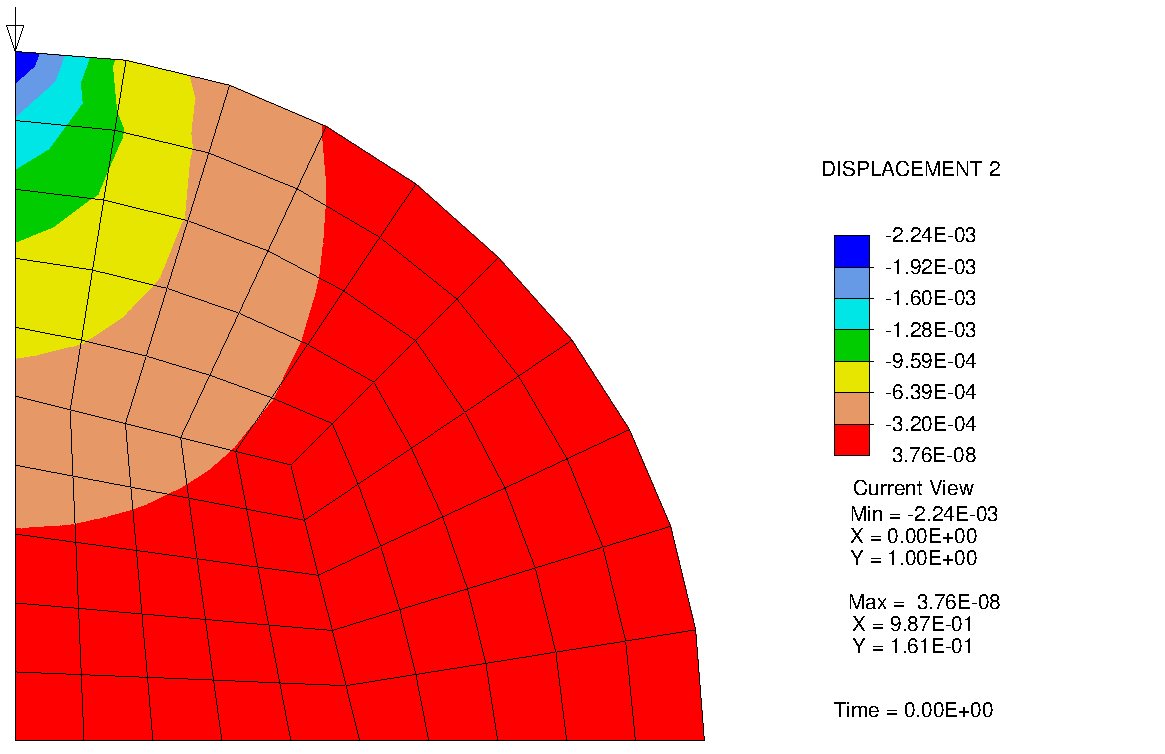
\includegraphics[width=4.2in]{figs/fig5} \hfil}
\caption{Contours of Vertical Displacement for Circular Disk}
\label{fig8}
\end{figure}

\section{Example 4. Strip with Hole and Slit.}
\label{ex4}

As a next example we consider the analysis of a tension strip which
contains a hole but has a slit between the hole and the right boundary
as shown in Figure \ref{fig9}.  The strip is to be loaded by applying vertical
displacements along the top and bottom.  The possibility of having
different materials for the top and bottom halves is anticipated and,
thus, the entire mesh needs to be constructed.

\begin{figure}[ht!]
\centerline {\hfil 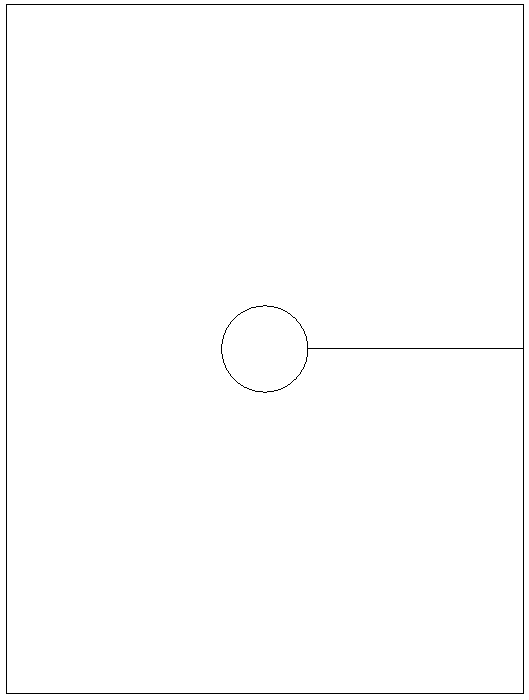
\includegraphics[width=1.6in]{figs/figo3} \hfil}
\caption{Tension Strip with Hole and Slit}
\label{fig9}
\end{figure}

To construct the mesh a set of 8 blocks of nodes and elements
will be constructed and merged to form the final analysis.  Since the mesh
has a considerable amount of symmetry it is proposed to generate the
two blocks for one quadrant using the {\tt BLOC}k mesh command
and then use  the {\tt TRAN}sformation command to form the other
quadrants.  The steps to form the mesh may be summarized as follows.
\begin{enumerate}
\item
Assign {\tt REGI}on 1 as the first quadrant.
\item
Use the {\tt BLOC}k command to form the two blocks for the first quadrant.
Save the mesh for the first quadrant in a file called {\tt IHQUAD}.
\item
Use an {\tt INCL}ude, {\tt IHQUAD} in a master data file (e.g., file
{\tt ISTRIP}) to import the data for quadrant 1 (see Chapter \ref{record}
for more information on use of the include option.
\item
Assign the second and third quadrants to {\tt REGI}on 2.
\item
Set the {\tt TRAN}sformation to reflect the x-axis and use an
{\tt INCL}ude, {tt\ IHQUAD} to generate the 2 blocks for the second
quadrant.  Note that since the coordinate transformation is not
a rotation the generated elements may have negative volume.
\item
Set the {\tt TRAN}s\-form\-a\-tion to reflect the x-axis and y-axes.
Use an {\tt INCL}\-ude, {\tt IHQUAD} to generate the 2 blocks for the third
quadrant.
\item
Assign the fourth quadrants to {\tt REGI}on 3.
\item
Set the {\tt TRAN}sformation to reflect y-axes.
Use an {\tt INCL}ude, {\tt IHQUAD} to generate the 2 blocks for the fourth
quadrant.
\end{enumerate}
The commands to perform the transformations and read the include files
are summarized in Figure \ref{fig10}.

\begin{figure}
\begin{verbatim}
       FEAPpv * * Tension Strip With Hole and Slit
       0,0,0,2,2,4
       PARAmeters
         d=1            ! First node number
         e=1            ! First element number
         m=1            ! Material set number
         n=8            ! Size of blocks
                        ! Terminator
       REGIon,1         ! Assigns 1st quadrant to region 1
         INCLude,IHQUAD ! Input first quadrant
       PARAmeters
         d=0            ! To make feap count nodes
         e=0            ! To make feap count elements
                        ! Terminator
       REGIon,2         ! Assign 2nd and 3rd quadrant
         TRANsform      ! Reverse x axis for second quadrant
           -1,0,0
            0,1,0
            0,0,1
            0,0,0
         INCLude,IHQUAD
         TRANsform ! Reverse x,y axis for third quadrant
           -1,0,0
            0,-1,0
            0,0,1
            0,0,0
         INCLude,IHQUAD
       REGIon,3    ! Assign 4th quadrant to region 3
         TRANsform ! Reverse y axis for fourth quadrant
            1,0,0
            0,-1,0
            0,0,1
            0,0,0
         INCLude,IHQUAD
       END
\end{verbatim}
\caption{Region, Transformation, and Include Structure}
\label{fig10}
\end{figure}

The outlines for all the blocks formed after this step are shown in
Figure \ref{fig11}.  It is necessary now to merge these blocks to form the
final mesh, while retaining the slit, which if not properly treated
will be merged also during the use of a {\tt TIE} command.

\begin{figure}[ht!]
\centerline {\hfil 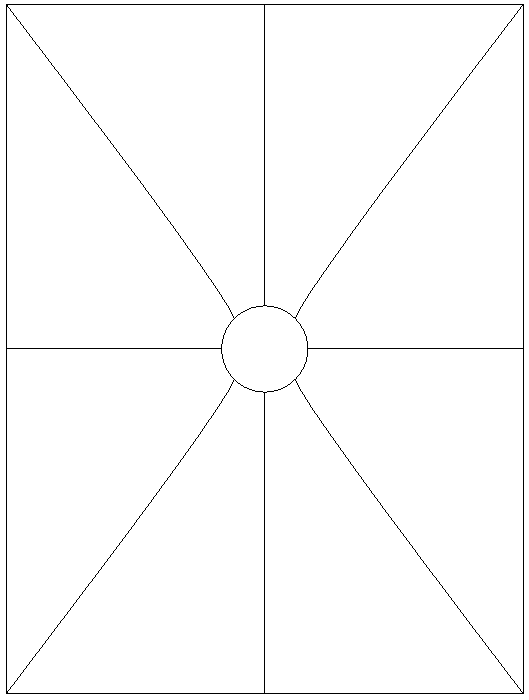
\includegraphics[width=1.6in]{figs/figo1} \hfil}
\caption{Tension Strip: Block Structure Before Merges}
\label{fig11}
\end{figure}

It is at this time that the utility of the {\tt REGI}on descriptions is
used.  A summary of the merge order is as follows

\begin{enumerate}
\item
Merge each of the regions with itself.  The result of this step is shown
in Figure \ref{fig12}.
\item
Merge region 1 with region 2; also merge region 2 with region 3.
This will produce the final mesh whose outline was shown in Figure \ref{fig9}.
\end{enumerate}
The {\tt TIE} commands to achieve these two steps are:
\begin{verbatim}
       TIE,REGIon,1,1
       TIE,REGIon,2,2
       TIE,REGIon,3,3
       TIE,REGIon,1,2
       TIE,REGIon,2,3
\end{verbatim}

\begin{figure}[ht!]
\centerline {\hfil 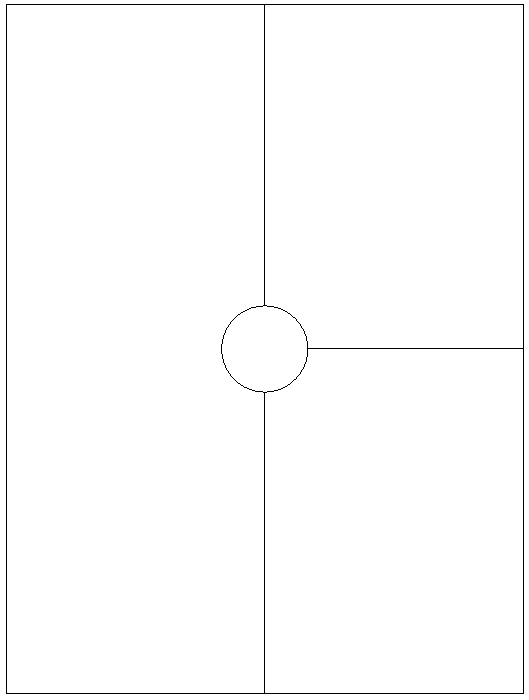
\includegraphics[width=1.6in]{figs/figo2} \hfil}
\caption{Tension Strip: After Merge of Each Region with Itself}
\label{fig12}
\end{figure}
The  generation of the two blocks forming each quadrant
is achieved using the commands shown
in Figure \ref{fig13} and after adding material properties and boundary
conditions an analysis produced the results for the $\sigma_{yy}$ stress
shown in Figure \ref{fig14}.

\begin{figure}
\begin{verbatim}
       PARAm
         p=atan(1.0)    ! 45-degrees in radians
         c=cos(p)
         s=sin(p)
         a=cos(0.5*p)
         b=sin(0.5*p)
                  ! Termination
       BLOCk
         CART,n,n,d,e,m
         1,1,0
         2,6,0
         3,6,8
         4,s,c
         5,2.6,0
         7,2.1,2.8
         8,a,b
         9,2.5,1.2
                  ! Termination
       BLOCk
         CART,n,n,0,0,m
         1,s,c
         2,6,8
         3,0,8
         4,0,1
         5,2.1,2.8
         7,0,3.1
         8,b,a
         9,1.1,3.0
                  ! Termination
\end{verbatim}
\caption{Tension Strip with Slit: Block Generation of Quadrant}
\label{fig13}
\end{figure}

\begin{figure}
\vbox{
\centerline {\hfil 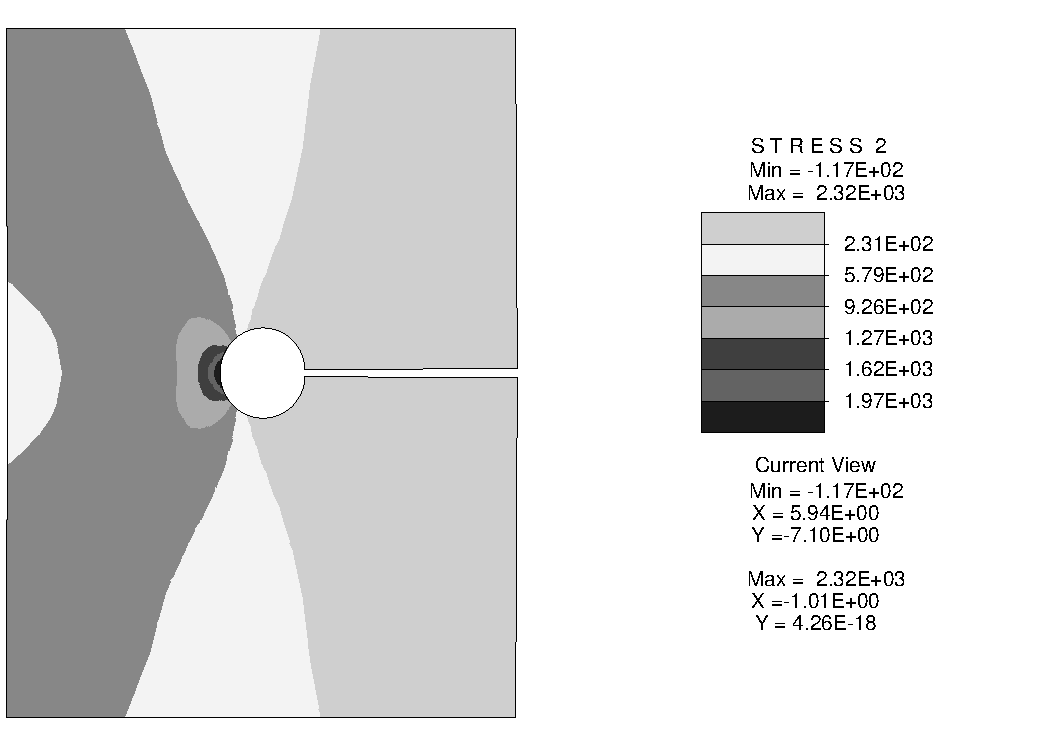
\includegraphics[width=4.2in]{figs/figo4} \hfil}
\caption{Tension Strip with Slit: Contours of $\sigma_{yy}$}
}
\label{fig14}
\end{figure}
